\documentclass{article}
\usepackage{tikz}

\begin{document}

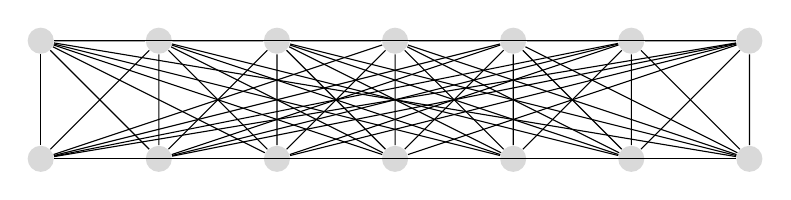
\begin{tikzpicture}[scale=1.5]
    % Define nodes
    \foreach \x in {0,...,6} {
        \pgfmathsetmacro{\y}{mod(\x+2, 7)}
        \node[circle, fill=gray!30] (n\x) at (\x, 0) {};
        \node[circle, fill=gray!30] (m\x) at (\y, 1) {};
    }
    
    % Draw edges
    \foreach \x in {0,...,6} {
        \pgfmathtruncatemacro{\nextx}{int(mod(\x+1, 7))}
        \draw (n\x) -- (n\nextx);
        \draw (m\x) -- (m\nextx);
        \draw (n\x) -- (m\nextx);
    }
    
    \foreach \x in {0,...,6} {
        \pgfmathtruncatemacro{\nextx}{int(mod(\x+2, 7))}
        \draw (n\x) -- (m\nextx);
    }
    
    \foreach \x in {0,...,6} {
        \pgfmathtruncatemacro{\nextx}{int(mod(\x+3, 7))}
        \draw (n\x) -- (m\nextx);
    }
    
    \foreach \x in {0,...,6} {
        \pgfmathtruncatemacro{\nextx}{int(mod(\x+4, 7))}
        \draw (n\x) -- (m\nextx);
    }
    
    \foreach \x in {0,...,6} {
        \pgfmathtruncatemacro{\nextx}{int(mod(\x+5, 7))}
        \draw (n\x) -- (m\nextx);
    }
    
    \foreach \x in {0,...,6} {
        \pgfmathtruncatemacro{\nextx}{int(mod(\x+6, 7))}
        \draw (n\x) -- (m\nextx);
    }
\end{tikzpicture}

\end{document}